\documentclass[twoside,a4wide,11pt]{article}\usepackage[]{graphicx}\usepackage[]{color}
%% maxwidth is the original width if it is less than linewidth
%% otherwise use linewidth (to make sure the graphics do not exceed the margin)
\makeatletter
\def\maxwidth{ %
  \ifdim\Gin@nat@width>\linewidth
    \linewidth
  \else
    \Gin@nat@width
  \fi
}
\makeatother

\definecolor{fgcolor}{rgb}{0.345, 0.345, 0.345}
\newcommand{\hlnum}[1]{\textcolor[rgb]{0.686,0.059,0.569}{#1}}%
\newcommand{\hlstr}[1]{\textcolor[rgb]{0.192,0.494,0.8}{#1}}%
\newcommand{\hlcom}[1]{\textcolor[rgb]{0.678,0.584,0.686}{\textit{#1}}}%
\newcommand{\hlopt}[1]{\textcolor[rgb]{0,0,0}{#1}}%
\newcommand{\hlstd}[1]{\textcolor[rgb]{0.345,0.345,0.345}{#1}}%
\newcommand{\hlkwa}[1]{\textcolor[rgb]{0.161,0.373,0.58}{\textbf{#1}}}%
\newcommand{\hlkwb}[1]{\textcolor[rgb]{0.69,0.353,0.396}{#1}}%
\newcommand{\hlkwc}[1]{\textcolor[rgb]{0.333,0.667,0.333}{#1}}%
\newcommand{\hlkwd}[1]{\textcolor[rgb]{0.737,0.353,0.396}{\textbf{#1}}}%
\let\hlipl\hlkwb

\usepackage{framed}
\makeatletter
\newenvironment{kframe}{%
 \def\at@end@of@kframe{}%
 \ifinner\ifhmode%
  \def\at@end@of@kframe{\end{minipage}}%
  \begin{minipage}{\columnwidth}%
 \fi\fi%
 \def\FrameCommand##1{\hskip\@totalleftmargin \hskip-\fboxsep
 \colorbox{shadecolor}{##1}\hskip-\fboxsep
     % There is no \\@totalrightmargin, so:
     \hskip-\linewidth \hskip-\@totalleftmargin \hskip\columnwidth}%
 \MakeFramed {\advance\hsize-\width
   \@totalleftmargin\z@ \linewidth\hsize
   \@setminipage}}%
 {\par\unskip\endMakeFramed%
 \at@end@of@kframe}
\makeatother

\definecolor{shadecolor}{rgb}{.97, .97, .97}
\definecolor{messagecolor}{rgb}{0, 0, 0}
\definecolor{warningcolor}{rgb}{1, 0, 1}
\definecolor{errorcolor}{rgb}{1, 0, 0}
\newenvironment{knitrout}{}{} % an empty environment to be redefined in TeX

\usepackage{alltt}
\usepackage[left=2.5cm,top=2cm,right=2cm,bottom=2.5cm,bindingoffset=0.5cm]{geometry}
\usepackage{amsmath} 
\usepackage[affil-it]{authblk}
\usepackage{hyperref}
\usepackage{fullpage}
\usepackage{pdflscape}
\usepackage[backend=bibtex,sorting=none,style=ieee]{biblatex}
\usepackage{setspace}
\usepackage{inconsolata}
\bibliography{chromothripsis}

\title{ShatterSeek: an R package for the detection of chromothripsis from Next-Generation Sequencing (NGS) data}
%structural rearrangements and copy number data

\author[1,2,3]{\rm Isidro Cortes-Ciriano}%\thanks{isidrolauscher@gmail.com}} 
\author[4]{\rm Ruibin Xi}%\thanks{ruibinxi@math.pku.edu.cn}}
\author[1,2]{\rm Peter J. Park\thanks{peter\_park@hms.harvard.edu}}

\affil[1]{Department of Biomedical Informatics, Harvard Medical School, Boston, Massachusetts, USA}
\affil[2]{Ludwig Center at Harvard, Boston, MA 02115, USA}
\affil[3]{Centre for Molecular Science Informatics, Department of Chemistry, University of Cambridge, Lensfield Road, Cambridge CB2 1EW, United Kingdom}
\affil[4]{School of Mathematical Sciences and Center for Statistical Science, Peking University, Beijing 100871, China}
\setlength{\parindent}{0pt}
\setlength{\parskip}{\baselineskip}

%--------------------------------------------------------------------------------
\IfFileExists{upquote.sty}{\usepackage{upquote}}{}
\begin{document}
%--------------------------------------------------------------------------------
\maketitle
\tableofcontents
\onehalfspacing

%-------------------------
\section{Introduction} %from Next-Generation Sequencing (NGS) data}
%-------------------------
Chromothripsis refers to the genomic alterations characterized by massive de novo rearrangements, 
often generated in a single catastrophic event, where the DNA is shattered into a number of 
fragments that are subsequently stitched together in random order and orientation. 
Chromothripsis can be confined to small chromosomal regions or can affect multiple chromosomes,
and can involve from tens to hundreds of rearrangements \cite{Stephens2011}.
Therefore, chromothripsis represents a mechanism for the accrual of tens to hundreds of rearrangements in a few cell divisions.\\
\\
Chromothripsis regions are characterized by copy number (CN) profiles oscillating between two or three states,
(in cases where partial duplications follow chromothripsis), 
interspersed loss of heterozygosity (LOH), 
and clusters of interleaved structural variations (SVs), 
where the proportions of fragment joins (i.e., duplication-like, deletion-like, head-to-head and tail-to-tail inversions) are roughly equal, consistent with the random stitching of genomic fragments through mostly non-homologous end-joining (NHEJ) DNA repair (Figure 1).\\
\\
Initial studies used array-derived copy number profiles to detect chromothripsis, 
as the amount of whole-genome sequencing data sets was limited \cite{Kim2013,Cai2014}.
%thus preventing to 
SNP arrays do not permit to fully characterize the genome-wide landscape of structural rearrangements at
single-base resolution, notably interchromosomal events.
%and hence,characterize the types of SVs comprised in regions subject to chromothripsis.
Hence, the detection of chromothripsis is more accurate  
if structural rearrangements and copy number data are integrated \cite{Notta2016,Li2014,Korbel2013,Govind2014}.
% The increasing amount of whole-genome sequencing data sets 
% thus requires the development of easy-to-use pipelines to detect chromothripsis from NGS data.

Korbel and Campbell \cite{Korbel2013} proposed a set of statistical criteria for the detection of chromothripsis that have been widely used in the literature. 
To date, there exist two publicly available packages for the detection of chromothripsis, namely: 
CTLP scanner \cite{Cai2014,Yang2016} and Shatterproof \cite{Govind2014}.
The former uses SNP array data, whereas the latter both copy number variation (CNV) and SV data.\\
\\
We have developed ShatterSeek, an R package that integrates copy number and SV data for the detection and 
visualization of chromothripsis events from NGS data.
ShatterSeek implements a custom graph-based approach to identify candidate chromothripsis regions, 
and then applies a set of statistical criteria based on Korbel and Campbell \cite{Korbel2013}
to detect both single and multichromosomal chromothripsis events.
In addition, ShatterSeek provides functionalities for the easy visualization of SVs, 
as well as CN and LOH profiles.
Visual inspection of candidate chromothripsis regions is still required in a number of cases due to the complexity of the observed events, and the overlapping features of chromothripsis and other complex events.
% ShatterSeek was validated using experimental daa
% comparison Shatterproof
We have recently validated ShatterSeek in a large-scale
study of ca. 2,600 cancer genomes and
shown its higher sensitivity and specificity with respect to Shatterproof.
We refer the reader to this work for further details about the rates and characteristics of chromothripsis across diverse human cancers.
The chromothripsis calls for all these tumors generated using ShatterSeek can be accessed at 
http://compbio.med.harvard.edu/chromothripsis/ \\
\\
In the next sections, we explain in detail the statistical criteria implemented in ShatterSeek to detect
chromothripsis events,
and illustrate its functionalities using data from a kidney renal cell carcinoma patient.

%-------------------------
\section{Workflow implemented in ShatterSeek}
%-------------------------
To identify chromothripsis-like patterns in cancer genomes, we implemented and extended 
the set of  criteria proposed by Campbell and Korbel \cite{Korbel2013}. 
The pipeline to detect chromothripsis consists of three major steps, namely:
(i) discovery of clusters of interleaved SVs using a graph-based approach,
(ii) evaluation of a set of statistical criteria in the genomic regions spanned by these clusters,
and (iii) evaluation of whether chromothripsis is confined to a single or to multiple chromosomes.\\
\\

\begin{figure}[htb]
\begin{center}
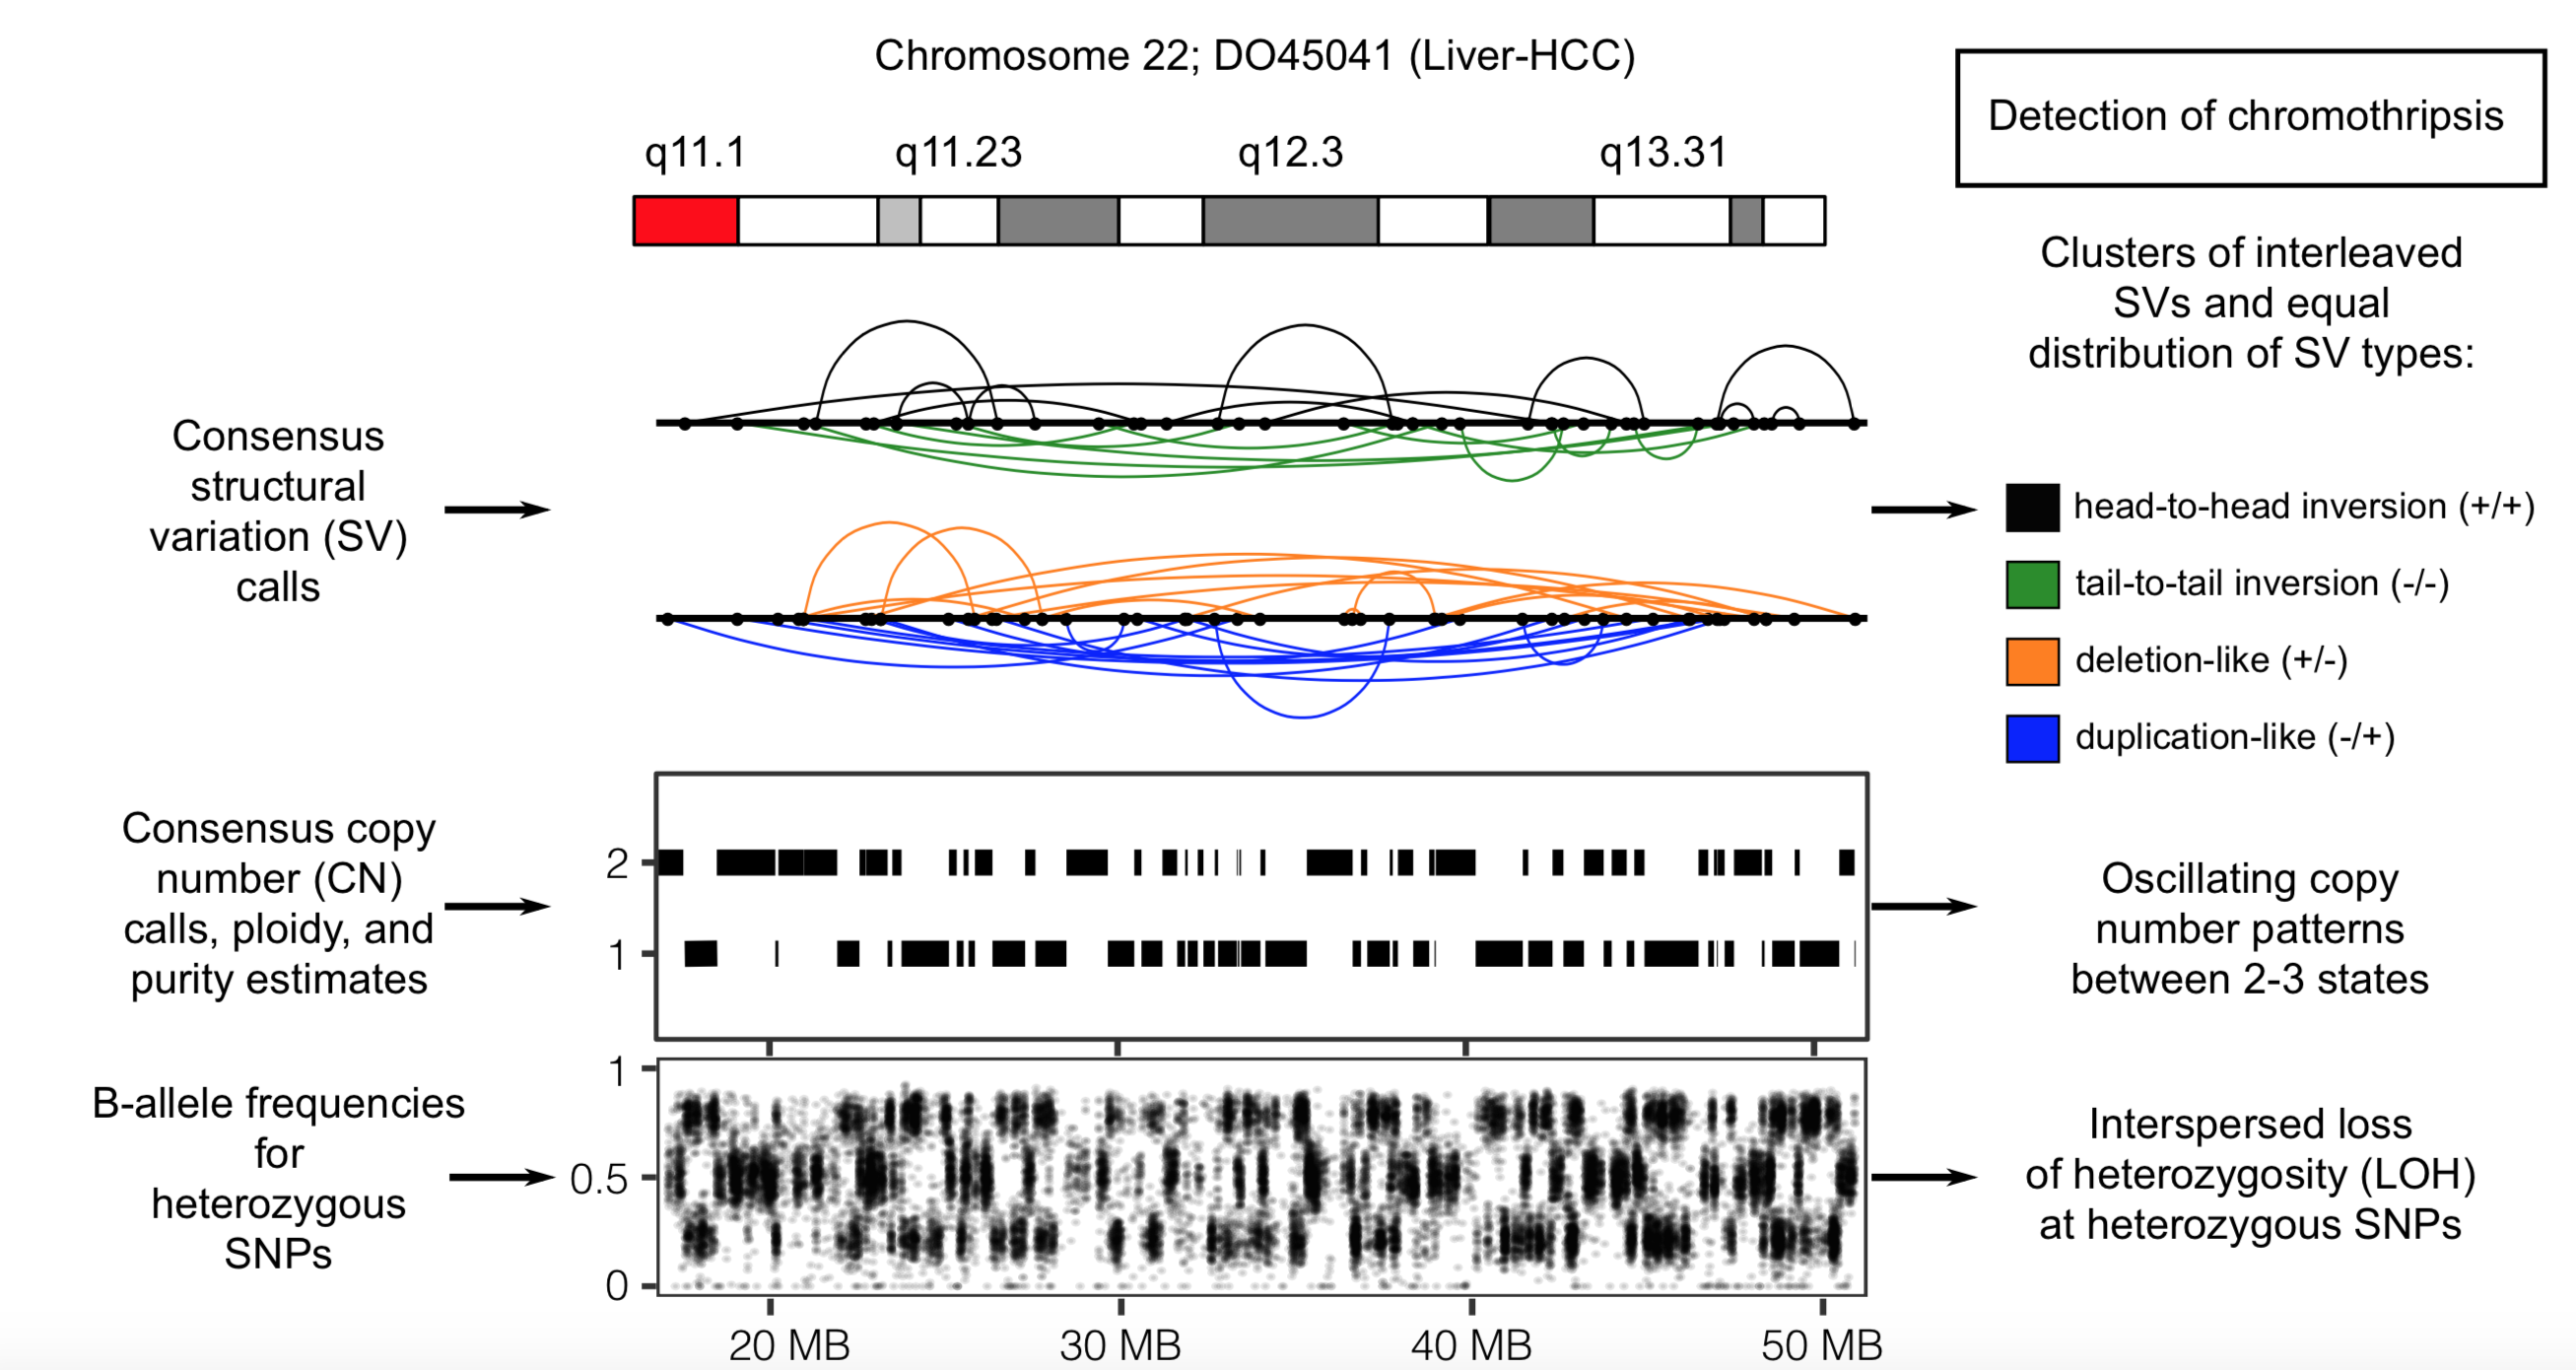
\includegraphics[width=\textwidth]{workflow_tutorial.png}
\caption{Illustrative example of chromothripsis and workflow and criteria used to detect chromothripsis events by ShatterSeek}
\end{center}
\end{figure}

\subsection{Detection of clusters of interleaved SVs}

Given that chromothripsis events generate clusters of interleaved rearrangements, 
we f
ShatterSeek firstly scans the cancer genomes for the presence of clusters of interleaved SVs,
which are expected to be generated by the random fragmentation and stitching of the genome.
We consider that two SVs are interleaved if the genomic regions bridged by their breakpoints overlap but are not nested. 
To find clusters within a given chromosome, 
ShatterSeek constructs an undirected graph using intrachromosomal SVs 
whose nodes correspond to SVs and whose edges connect interleaved SVs. 
Thus, clusters of SVs can be detected by finding the connected components in the graph. 
The connected component in each chromosome with the highest number of SVs is considered for further analysis. 
By default, ShatterSeek only considers chromosomes 1-22 and X.
In the following, we use the term {\it chromothripsis region} to refer to the genomic regions affected by chromothripsis within one chromosome, whereas we term {\it chromothripsis event} the set of chromothripsis regions involved in a single catastrophic event.
Thus, a chromothripsis event can affect a single chromosome, multiple regions within a chromosome, or comprise genomic regions from multiple chromosomes.

\subsection{Statistical criteria implemented in ShatterSeek}

Once the clusters of interleaved SVs are detected, ShatterSeek evaluates the following statistical criteria following the work by Korbel and Campbell \cite{Korbel2013}.

% We decided to only consider the criteria of loss of heterozygosity proposed by (Korbel and Campbell, 2013) when examining the set of canonical chromothripsis calls detected in diploid genomes. We did not consider this criterion to call chromothripsis across the entire tumor cohort because we noticed that some bona fide chromothripsis cases identified in low-purity samples (e.g., Figure 2c) might not meet the cut-off for statistical significance due to the infiltration of normal tissue. In such a case, the allelic ratios (i.e., B allele frequencies) for heterozygous SNPs would not divert significantly from 0.5, and thus, would hamper the observation of alternating LOH patterns associated to copy losses (Song et al., 2012). This phenomenon is exacerbated when chromothripsis occurs in aneuploid tumors due to increased CN, and hence, chromothripsis events do not necessarily lead to LOH (see e.g., Supplementary Figure 5C).

\subsubsection{Equal distribution of SV types}

Once the SV clusters are detected, ShatterSeek evaluates whether the distribution of DNA fragment joins,
i.e., deletion-like (+/-; or "head"/"tail"), duplication-like (-/+), head-to-head (+/+), and tail-to-tail (-/-) inversions,
diverges from a multinomial distribution with equal probabilities for each SV category using the goodness-of-fit test for the multinomial distribution from the R package stats (chiq.test function).
The types of SVs are determined by the orientation of the reads mapped to the breakpoints (see \cite{Zhang2013} for further details).
We term this test 'fragment joins test'.

\subsubsection{Chromosomal enrichment of breakpoints}
Massive chromothripsis events, which involve hundreds of SVs,
generally affect large genomic regions in one or multiple chromosomes against the background of 
quiescent genomes.
Thus, in these cases the chromosomes harboring chromothripsis are highly enriched for breakpoints.
An example of a chromothripsis event is depicted in Figure 1.
We term this test 'chromosomal breakpoint enrichment test'.

To test for the enrichment of breakpoints in each chromosome,
ShatterSeek uses the binomial test corrected for mappability. 
We note that this test might be misleading for focal chromothripsis events
appearing in highly rearranged genomes, where
other chromosomes not displaying chromothripsis harbor a number of SVs (interleaved or not) comparable to that
detected in chromosomes displaying chromothripsis. 
Therefore, this criterion needs to be interpreted carefully on a per-case basis (please see below).

\subsubsection{Random distribution of breakpoints}
ShatterSeek also evaluates whether the distribution of the breakpoints comprised in the SV clusters
differs from an exponential distribution, as described by Korbel and Campbell \cite{Korbel2013}.
We term this test 'random distribution of breakpoints test'.

\subsubsection{Number of oscillating copy number segments}
A hallmark of chromothripsis is the 
presence of copy number profiles oscillating between two or three copy number states.
This feature has been widely used before to detect chromothripsis from 
genome-wide copy number profiles using operational definitions,
e.g., at least 10 contiguous segments oscillating between two copy number states \cite{Rausch2012}. 

To uncover oscillating patterns in the genomic regions delimited by the distal breakpoints composing 
the clusters of interleaved SVs,
ShatterSeek reports the number of uninterrupted CN segments oscillating across 2 and 3 states.
% contiguous genomic segments oscillate between two or three CN states.

\subsubsection{Interspersed loss of heterozygosity (LOH)}

We decided not to use the criterion of loss of heterozygosity proposed by Campbell and Korbel \cite{Korbel2013}, 
as we noticed that in some bona fide chromothripsis cases identified in low-purity samples 
In LOH regions, the allelic ratios for heterozygous SNPs (i.e., B allele frequencies or BAF) are either 1 or 0.
However, in low-purity tumor samples, where the fraction of cancer cells is reduced,
the infiltration of normal tissue heavily distorts the B allele frequencies (BAF) profile of the tumor.
Hence, this limits the power to detect significant changes due to LOH in the BAF profile. 
In such cases, the BAF values would not divert significantly from 0.5 even in LOH regions, and thus, would hamper the observation of alternating LOH patterns associated to copy losses \cite{Song2012}.
In addition, assessing LOH in aneuploid tumors is often difficult,
where the BAF values for oscillating segments between high CN levels do not vary strongly.\\
% Please see Figure X for an example of a chromothripsis event detected in a low-purity tumor where the BAF 
% profile does not oscillate \\
\\
However, given that the loss of heterozygosity profiles are very useful to
determine the temporal profile of chromothripsis events, 
and to distinguish chromothripsis from chromoanasynthesis in nearly-diploid cases,
ShatterSeek provides capabilities to visualize LOH/CN minor profiles at chromothripsis regions.
\\

\subsection{Detection of multichromosomal chromothripsis events}
ShatterSeek considers that two or more  chromothripsis regions belong to the same 
catastrophic event if these regions +/- 10Kb (default value) are linked by at least two interchromosomal SVs.
Given that the sensitivity of SV detection algorithms is still limited,
it is not always possible to detect rearrangements between all regions belonging to the same chromothripsis event.
Thus, in cases where at least three chromosomes were involved, 
ShatterSeek applies transitive reasoning to identify the full extent of the events. 
For instance, if the chromothripsis regions detected in chromosomes 1 and 2 are linked, and those detected in chromosome 2 are also linked to a chromothripsis region in chromosome 3, ShatterSeek considers that the chromothripsis patterns detected in these three chromosomes were generated as a result of the same catastrophic event.

% The P values from these three tests were corrected using the FDR method. The level of significance was set to q ≤ 0.2. 
% Finally, the genomic regions delimited by the distal breakpoints composing the clusters of interleaved SVs were further examined for the presence of contiguous genomic segments oscillating between two CN states. 


%-----------------------------------------------------------------------------------------------------
\section{Recommended cut-off values to interpret the output of ShatterSeek}

After manual curation of hundreds of massive and focal chromothripsis calls, 
we derived the following guidelines to detect chromothripsis using Shatteseek.

We assign two levels of confidence depending on the set of statistical tests
satisfied by a candidate chromothripsis region.
% consider as high-confidence chromothripsis regions those satisfying at least one of the
% two first sets of cut-off values for the statistical criteria described above:

\begin{itemize}

\item High confidence: at least 6 interleaved intrachromosomal SVs, 7 contiguous segments oscillating between 2 CN states, 
the fragment joins test, and either the chromosomal enrichment or the exponential distribution of breakpoints test.

\item High confidence: at least 3 interleaved intrachromosomal SVs and 4 or more interchromosomal SVs, 7 contiguous segments oscillating between 2 CN states and the fragment joins test.

\item Low confidence: at least 6 interleaved intrachromosomal SVs, 4, 5 or 6 adjacent segments oscillating between 2 CN states, the fragment joins test, and either the chromosomal enrichment or the exponential distribution of breakpoints test.

\end{itemize}

% T(following the criteria previously used )
Application of these criteria to ~2,600 whole genomes still led to a small set of false positives that were removed by visual inspection. 
This is mostly due to the fact that multiple layers of rearragements other than chromothripsis might coexist, and the aggregate of these might satisfy the statistical tests described above.
In addition, chromothripsis regions are highly heterogeneous, running the gamut from massive chromothripsis cases 
invovling hundreds of SVs in an otherwise quiescent genome, 
to focal events in the context of genomes highly rearranged by other mutational processes.
This heterogeneity makes it almost impossible to define a set of criteria with perfect
discriminative power for chromothripsis.
Therefore, we advocate, as far as possible, for the manual curation of candidate chromothripsis regions. 
To facilitate this process, ShatterSeek provides functionalities to visually depict the candidate chromothripsis regions (see below). 


%------------------------------------------------------------------------------------------------------
\section{How to use ShatterSeek}
%------------------------------------------------------------------------------------------------------
In the following sections, we illustrate how to install and use ShatterSeek to detect and visualize chromothripsis 
using SV and CNV data. 
This tutorial assumes minimal knowledge of the R programming language.

\subsection{Installation}
ShatterSeek is entirely written in R. 
To install ShatterSeek type the following in R: 
\begin{knitrout}
\definecolor{shadecolor}{rgb}{0.969, 0.969, 0.969}\color{fgcolor}\begin{kframe}
\begin{alltt}
\hlkwd{require}\hlstd{(devtools)}
\hlkwd{install_github}\hlstd{(}\hlstr{"parklab/ShatterSeek"}\hlstd{)}
\end{alltt}
\end{kframe}
\end{knitrout}
Alternatively, please download the latest release of ShatterSeek by running in a bash terminal:\\
\begin{knitrout}
\definecolor{shadecolor}{rgb}{0.969, 0.969, 0.969}\color{fgcolor}\begin{kframe}
\begin{alltt}
git clone git@github.com:parklab/ShatterSeek.git 
unzip ShatterSeek-master.zip 
R CMD INSTALL ShatterSeek-master
\end{alltt}
\end{kframe}
\end{knitrout}

% To install the development branch of ShatterSeek please run:\\
% <<engine='bash',eval=FALSE>>=
% wget XX
% unzip
% R CMD INSTALL XX
% @

\subsection{Load SV and CNV data into R}

% XX data from any caller can be used
% XX ein PCAWG consensus, etc.. 
% XX total copy number in integer format (output of e.g. ASCAT)

We first load ShatterSeek and the test data that is provided with the package.
This corresponds to the SV and CN data for a kidney renal cell carcinoma tumor (ICGC ID: DO17373).
The chromothipsis events detected in this tumor sample are depicted in Figure 2. The other
chromosomes in this tumor showed unaltered CN profiles with respect to the normal tissue sample.

\begin{knitrout}
\definecolor{shadecolor}{rgb}{0.969, 0.969, 0.969}\color{fgcolor}\begin{kframe}
\begin{alltt}
\hlkwd{library}\hlstd{(ShatterSeek)}
\hlkwd{data}\hlstd{(DO17373)}
\end{alltt}
\end{kframe}
\end{knitrout}
Running this command loads to the workspace two R dataframes, corresponding to the somatic SVs (SV\_DO17373)
and CN (SCNA\_DO17373) calls for this tumor.
These calls are consensus calls generated by the Pan-Cancer Analysis of Whole Genomes (PCAWG) project.
ShatterSeek accepts CN and SV calls from any caller, 
provided they are encoded in the format required by ShatterSeek (please see below).
However, we note that the sensitivity of ShatterSeek depends on the quality of the SV and CN calls used.
Hence, it is the responsability of the user to guarantee that the SV and CN calls are of sufficient quality.

\begin{figure}[!htb]
\begin{center}
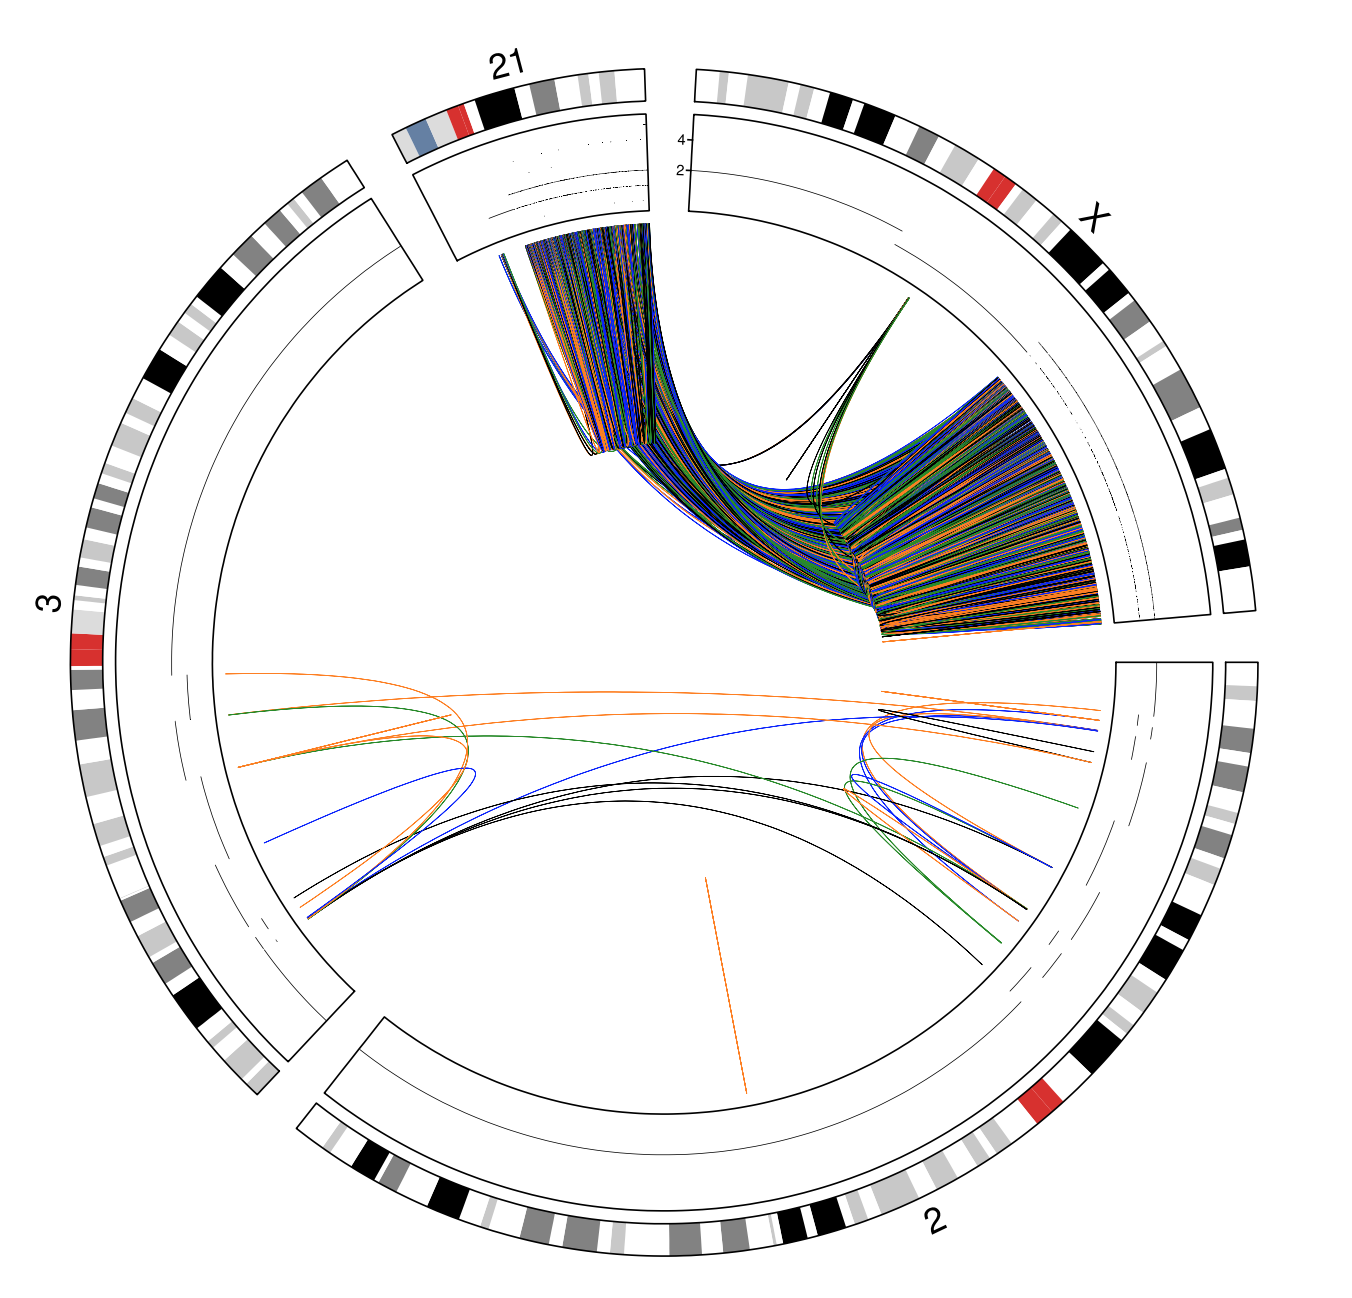
\includegraphics[width=9cm,height=9cm]{2939_massive.png}
\caption{Evidence of two massive multichromosomal chromothripsis events involving 
chromosomes 21-X and 2-3 detected in a kidney renal cell carcinoma tumor in patient DO17373 (TCGA-CJ-5681).}
\end{center}
\end{figure}


ShatterSeek requires the SV data to be stored in a data.frame with the following columns: 
\begin{itemize}
\item chrom1 (character): chromosome for the first breakpoint
\item pos1 (character): position for the first breakpoint
\item chrom2 (character): chromosome for the second breakpoint 
\item pos2 (character): position for the second breakpoint
\item SVtype (character): type of SV, encoded as: DEL (deletion-like; +/-), DUP (duplication-like; -/+),
h2hINV (head-to-head inversion; +/+), and t2tINV (tail-to-tail inversion; -/-).
\item strand1 (e.g. + for DEL)
\item strand2 (e.g. - for DEL)
\end{itemize}
Chromosomes are expected to be in Ensembl chromosome notation, i.e. NOT contain the prefix "chr".\\
\begin{knitrout}
\definecolor{shadecolor}{rgb}{0.969, 0.969, 0.969}\color{fgcolor}\begin{kframe}
\begin{alltt}
\hlkwd{head}\hlstd{(SV_DO17373)}
\end{alltt}
\begin{verbatim}
##   chrom1    start1      end1 chrom2   start2     end2       sv_id
## 1      1 142618685 142618686     21 21708092 21708093 SVMERGE1159
## 2      1 142623413 142623414     21 25233137 25233138  SVMERGE269
## 3      1 142639910 142639911     21 33703275 33703276  SVMERGE127
## 4      1 143536371 143536372     21 29698088 29698089 SVMERGE1343
## 5     11   8540384   8540385     11  8541772  8541773   SVMERGE55
## 6     14  61896353  61896354     14 62061595 62061596 SVMERGE1006
##   pe_support strand1 strand2 svclass                    svmethod
## 1         18       +       -     TRA               SNOWMAN_DELLY
## 2         50       -       -     TRA       SNOWMAN_dRANGER_DELLY
## 3         34       +       -     TRA             SNOWMAN_dRANGER
## 4         39       -       +     TRA             SNOWMAN_dRANGER
## 5         37       +       -     DEL         SNOWMAN_BRASS_DELLY
## 6        111       -       +     DUP SNOWMAN_BRASS_dRANGER_DELLY
\end{verbatim}
\end{kframe}
\end{knitrout}

Please remember that ShatterSeek only considers chromosomes 1-22 and X.
Thus, make sure that the SVs comprised in your input data only correspond to these chromosomes.
The SV data is loaded into an object of class "SV", using the function {\it SVs}:

\begin{knitrout}
\definecolor{shadecolor}{rgb}{0.969, 0.969, 0.969}\color{fgcolor}\begin{kframe}
\begin{alltt}
\hlstd{SV_data} \hlkwb{<-} \hlkwd{SVs}\hlstd{(}\hlkwc{chrom1}\hlstd{=}\hlkwd{as.character}\hlstd{(SV_DO17373}\hlopt{$}\hlstd{chrom1),}
                \hlkwc{pos1}\hlstd{=}\hlkwd{as.numeric}\hlstd{(SV_DO17373}\hlopt{$}\hlstd{start1),}
                \hlkwc{chrom2}\hlstd{=}\hlkwd{as.character}\hlstd{(SV_DO17373}\hlopt{$}\hlstd{chrom2),}
                \hlkwc{pos2}\hlstd{=}\hlkwd{as.numeric}\hlstd{(SV_DO17373}\hlopt{$}\hlstd{end2),}
                \hlkwc{SVtype}\hlstd{=}\hlkwd{as.character}\hlstd{(SV_DO17373}\hlopt{$}\hlstd{svclass),}
                \hlkwc{strand1}\hlstd{=}\hlkwd{as.character}\hlstd{(SV_DO17373}\hlopt{$}\hlstd{strand1),}
                \hlkwc{strand2}\hlstd{=}\hlkwd{as.character}\hlstd{(SV_DO17373}\hlopt{$}\hlstd{strand2))}
\end{alltt}
\end{kframe}
\end{knitrout}

ShatterSeek requires the CNV data to be in the following format:
(i)
\begin{itemize}
\item chrom (character): chromosome (also in Ensembl notation)
\item start (numeric): start position for the CN segment
\item end (numeric): end position for the CN segment
\item CN (numeric): integer total copy number (e.g. 2 for unaltered chromosomal regions)
\end{itemize}
\begin{knitrout}
\definecolor{shadecolor}{rgb}{0.969, 0.969, 0.969}\color{fgcolor}\begin{kframe}
\begin{alltt}
\hlkwd{head}\hlstd{(SCNA_DO17373)}
\end{alltt}
\begin{verbatim}
##   chromosome    start       end total_cn
## 1          1        1 249250620        2
## 3          2    20016  11969465        2
## 4          2 11969466  14420187        1
## 5          2 14420188  16916033        2
## 6          2 16916034  16937471        1
## 7          2 16937472  17054487        2
\end{verbatim}
\end{kframe}
\end{knitrout}

The CNV data is loaded into an object of class "CNVsegs", using the function {\it CNVsegs}:
\begin{knitrout}
\definecolor{shadecolor}{rgb}{0.969, 0.969, 0.969}\color{fgcolor}\begin{kframe}
\begin{alltt}
\hlstd{CN_data} \hlkwb{<-} \hlkwd{CNVsegs}\hlstd{(}\hlkwc{chrom}\hlstd{=}\hlkwd{as.character}\hlstd{(SCNA_DO17373}\hlopt{$}\hlstd{chromosome),}
                     \hlkwc{start}\hlstd{=SCNA_DO17373}\hlopt{$}\hlstd{start,}
                     \hlkwc{end}\hlstd{=SCNA_DO17373}\hlopt{$}\hlstd{end,}
                     \hlkwc{total_cn}\hlstd{=SCNA_DO17373}\hlopt{$}\hlstd{total_cn)}
\end{alltt}
\end{kframe}
\end{knitrout}

Once the input data has been loaded, we proceed to run the main function of the package,
namely {\it shatterseek}.
This function runs the code to detect clusters of interleaved SVs, 
and subsequently evaluates each candidate chromothripsis region for
the statistical criteria described above.

\begin{knitrout}
\definecolor{shadecolor}{rgb}{0.969, 0.969, 0.969}\color{fgcolor}\begin{kframe}
\begin{alltt}
\hlkwd{library}\hlstd{(ShatterSeek)}
\hlstd{start_time} \hlkwb{<-} \hlkwd{Sys.time}\hlstd{()}
\hlstd{chromothripsis} \hlkwb{<-} \hlkwd{shatterseek}\hlstd{(}\hlkwc{SV.sample}\hlstd{=SV_data,} \hlkwc{seg.sample}\hlstd{=CN_data)}
\end{alltt}
\begin{verbatim}
## Running..
## 
## 
## Evaluating the statistical criteria
## Successfully finished!
\end{verbatim}
\begin{alltt}
\hlstd{end_time} \hlkwb{<-} \hlkwd{Sys.time}\hlstd{()}
\hlkwd{print}\hlstd{(}\hlkwd{paste0}\hlstd{(}\hlstr{"Running time (s): "}\hlstd{,}\hlkwd{round}\hlstd{(end_time} \hlopt{-} \hlstd{start_time,}\hlkwc{digits}\hlstd{=}\hlnum{2}\hlstd{)))}
\end{alltt}
\begin{verbatim}
## [1] "Running time (s): 17.73"
\end{verbatim}
\begin{alltt}
\hlkwd{print}\hlstd{(}\hlkwd{head}\hlstd{(chromothripsis}\hlopt{@}\hlkwc{chromSummary}\hlstd{))}
\end{alltt}
\begin{verbatim}
##   chrom     start       end number_DEL number_DUP number_h2hINV
## 1     1        NA        NA          0          0             0
## 2     2  11969466  75460870          3          3             2
## 3     3  20704347  85709275          2          1             1
## 4     4        NA        NA          0          0             0
## 5     5 140129029 171935828          0          2             0
## 6     6        NA        NA          0          0             0
##   number_t2tINV number_TRA clusterSize_including_TRA number_SVs_sample
## 1             0          0                         0              1426
## 2             0          7                        15              1426
## 3             0          6                        10              1426
## 4             0          0                         0              1426
## 5             0          0                         2              1426
## 6             0          0                         0              1426
##   number_CNV_segments pval_fragment_joins chr_breakpoint_enrichment
## 1                  NA                  NA              8.612611e-17
## 2                  13           0.8653370              2.949495e-08
## 3                  14           0.5724067              1.185413e-07
## 4                  NA                  NA              1.852862e-17
## 5                   1           0.1116102              6.729654e-15
## 6                  NA                  NA              3.277719e-14
##   pval_exp_chr pval_exp_cluster
## 1           NA               NA
## 2 1.857513e-08     0.000000e+00
## 3 0.000000e+00     1.154479e-09
## 4           NA               NA
## 5           NA               NA
## 6           NA               NA
##   max_number_oscillating_CN_segments_2_states
## 1                                          NA
## 2                                          11
## 3                                          12
## 4                                          NA
## 5                                          NA
## 6                                          NA
##   max_number_oscillating_CN_segments_3_states number_CN_segments_chr
## 1                                          NA                     NA
## 2                                          11                     13
## 3                                          12                     13
## 4                                          NA                     NA
## 5                                          NA                     NA
## 6                                          NA                     NA
##   max_number_oscillating_CN_segments_2_states_chr
## 1                                              NA
## 2                                              13
## 3                                              13
## 4                                              NA
## 5                                              NA
## 6                                              NA
##   max_number_oscillating_CN_segments_3_states_chr inter_number_DEL
## 1                                              NA                0
## 2                                              13                4
## 3                                              13                4
## 4                                              NA                0
## 5                                              NA                0
## 6                                              NA                0
##   inter_number_h2hINV inter_number_t2tINV inter_number_DUP
## 1                   0                   0                0
## 2                   2                   3                2
## 3                   3                   4                3
## 4                   0                   0                0
## 5                   0                   0                0
## 6                   0                   0                0
##   inter_pval_fragment_joins inter_other_chroms
## 1                        NA                   
## 2                 0.8012520                  3
## 3                 0.9626925                  2
## 4                        NA                   
## 5                        NA                   
## 6                        NA                   
##   inter_other_chroms_coords_all
## 1                              
## 2          3:20704347-85709275;
## 3          2:11969466-75460870;
## 4                              
## 5                              
## 6
\end{verbatim}
\end{kframe}
\end{knitrout}

% <<echo=TRUE,results='hide',warning=FALSE,message=FALSE,eval=TRUE,tidy=TRUE,render=T>>=
% #chromothripsis@chromSummary 
% detach("package:ShatterSeek", unload=TRUE)
% library(ShatterSeek)
% @

The function {\it ShatterSeek} returns an instance of the 'chromoth' class that contains two slots, namely:
{\it detail} and {\it chromSummary}. 
The slot {\it detail} contains a list containing the input data (SV and CNV calls), 
as well as intermediate results obtained by running the graph-based approach
implemented to discover clusters of interleaved SVs:
\begin{knitrout}
\definecolor{shadecolor}{rgb}{0.969, 0.969, 0.969}\color{fgcolor}\begin{kframe}
\begin{alltt}
\hlkwd{names}\hlstd{(chromothripsis}\hlopt{@}\hlkwc{detail}\hlstd{)}
\end{alltt}
\begin{verbatim}
##  [1] "SV"             "graph"          "connComp"       "num.chromth"   
##  [5] "maxSVs"         "degree"         "numSVByChrom"   "maxClusterSize"
##  [9] "SVinter"        "CNV"
\end{verbatim}
\end{kframe}
\end{knitrout}

The slot {\it chromothripsis@chromSummary} is a data.frame where each row corresponds to a chromosome,
and the columns to the values of the statistical criteria and additional information.
The columns are:

\begin{itemize}
\item chrom: chromosome
\item start: start position for the cluster of interleaved SVs detected in chromosome 'chrom'
\item end: end position for the cluster of interleaved SVs detected in chromosome 'chrom'
\item number\_DEL: number of intrachromosomal deletion-like SVs (+/-) mapped within the cluster region 
\item number\_DUP: number of intrachromosomal duplication-like SVs (-/+) mapped within the cluster region
\item number\_h2hINV: number of intrachromosomal head-to-head SVs (+/+) mapped within the cluster region
\item number\_t2tINV: number of intrachromosomal tail-to-tail SVs (-/-) mapped within the cluster region
\item number\_TRA: number of interchromosomal SVs mapped within the cluster
\item clusterSize\_including\_TRA: total number of SVs (including inter- and intrachromosomal SVs) mapped to the cluster region
\item number\_SVs\_sample: total number of SVs (including inter- and intrachromosomal SVs) detected in the sample
\item number\_CNV\_segments: number of CN segments located within the cluster boundaries
\item pval\_fragment\_joins: P value for the fragment joins test considering only the intrachromsomal SVs mapped to the cluster region
\item chr\_breakpoint\_enrichment: P value for the "chromosomal breakpoint enrichment" test
\item pval\_exp\_chr: P value for the 'random distribution of breakpoints' test considering all breakpoints in the  chromosome
\item pval\_exp\_cluster: P value for the 'random distribution of breakpoints' test considering only the breakpoints mapped to the cluster region
\item max\_number\_oscillating\_CN\_segments\_2\_states: Maximum number of uninterrupted oscillations between 2 CN states in the cluster region
\item max\_number\_oscillating\_CN\_segments\_3\_states: Maximum number of uninterrupted oscillations across 3 CN states in the cluster region
\item number\_CN\_segments\_chr: number of CN segments in the chromosome 
\item max\_number\_oscillating\_CN\_segments\_2\_states\_chr: Maximum number of uninterrupted oscillations between 2 CN states in the chromosome
\item max\_number\_oscillating\_CN\_segments\_3\_states\_chr: Maximum number of uninterrupted oscillations across 3 CN states in the chromosome
\item inter\_number\_DEL: number of interchromosomal deletion-like SVs (+/-) with one breakpoint mapped within the cluster region
\item inter\_number\_DUP: number of interchromosomal duplication-like SVs (-/+) with one breakpoint mapped within the cluster region
\item inter\_number\_h2hINV: number of interchromosomal head-to-head SVs (+/+) with one breakpoint mapped within the cluster region
\item inter\_number\_t2tINV: number of interchromosomal tail-to-tail SVs (-/-) with one breakpoint mapped within the cluster region
\item inter\_pval\_fragment\_joins: P value for the fragment joins test considering the inter- and intrachromosomal SVs mapped to the cluster region
\item inter\_other\_chroms: chromosomes linked by at least 2 SVs with the cluster region detected in chromosome 'chrom'
\item inter\_other\_chroms\_coords\_all: chromosomal coordinates for the clusters of SVs detected in other chromosomes linked by at least 2 SVs with the cluster region detected in the chromosome under consideration (i.e. the one specified in 'chrom')
\end{itemize}






\section{Visualization of chromothripsis regions}

ShatterSeek provides functionalities to inspect the detected chromothripsis regions. 
The function {\it plot\_chromothripsis} takes as input the output of the function 
{\it ShatterSeek} and a chromosome number. 
It returns a list containing 4 ggplot objects:
\begin{itemize}
\item ideogram of the affected region (only hg19 is supported at the moment). 
\item Representatin of the SVs. SVs are depicted as arcs with the breakpoints represented by black points. 
The breakpoints corresponding to interchromosomal SVs are depicted as colored points.
Duplication-like SVs, deletion-like SVs, head-to-head and tail-to-tail inversions are depicted by default in blue, orange, black, and green, respectively.
\item Total CN profile. Each CN segment is represented by a black rectangle.
\item Information for the depicted region is given as a table.
\end{itemize} 

These four ggplot objects, which can be modified to tailor the user's needs, 
can be easily combined using the function {\it arrangeGrob} from the R package gridExtra,
and visualized using e.g. the function {\it plot\_grid} from the R package cowplot.

\begin{knitrout}
\definecolor{shadecolor}{rgb}{0.969, 0.969, 0.969}\color{fgcolor}\begin{kframe}
\begin{alltt}
\hlkwd{library}\hlstd{(gridExtra)}
\hlstd{plots_chr3} \hlkwb{=} \hlkwd{plot_chromothripsis}\hlstd{(}\hlkwc{ShatterSeek_output} \hlstd{= chromothripsis,}\hlkwc{chr} \hlstd{=} \hlstr{"3"}\hlstd{)}
\hlstd{plot_chr3} \hlkwb{=} \hlkwd{arrangeGrob}\hlstd{(plots_chr3[[}\hlnum{1}\hlstd{]],}
                        \hlstd{plots_chr3[[}\hlnum{2}\hlstd{]],}
                        \hlstd{plots_chr3[[}\hlnum{3}\hlstd{]],}
                        \hlstd{plots_chr3[[}\hlnum{4}\hlstd{]],}
                        \hlkwc{nrow}\hlstd{=}\hlnum{4}\hlstd{,}\hlkwc{ncol}\hlstd{=}\hlnum{1}\hlstd{,}\hlkwc{heights}\hlstd{=}\hlkwd{c}\hlstd{(}\hlnum{0.2}\hlstd{,}\hlnum{.4}\hlstd{,}\hlnum{.4}\hlstd{,}\hlnum{.4}\hlstd{))}

\hlstd{plots_chr2} \hlkwb{=} \hlkwd{plot_chromothripsis}\hlstd{(}\hlkwc{ShatterSeek_output} \hlstd{= chromothripsis,}\hlkwc{chr} \hlstd{=} \hlstr{"2"}\hlstd{)}
\hlstd{plot_chr2} \hlkwb{=} \hlkwd{arrangeGrob}\hlstd{(plots_chr2[[}\hlnum{1}\hlstd{]],}
                        \hlstd{plots_chr2[[}\hlnum{2}\hlstd{]],}
                        \hlstd{plots_chr2[[}\hlnum{3}\hlstd{]],}
                        \hlstd{plots_chr2[[}\hlnum{4}\hlstd{]],}
                         \hlkwc{nrow}\hlstd{=}\hlnum{4}\hlstd{,}\hlkwc{ncol}\hlstd{=}\hlnum{1}\hlstd{,}\hlkwc{heights}\hlstd{=}\hlkwd{c}\hlstd{(}\hlnum{0.2}\hlstd{,}\hlnum{.4}\hlstd{,}\hlnum{.4}\hlstd{,}\hlnum{.4}\hlstd{))}

\hlstd{plots_chr21} \hlkwb{=} \hlkwd{plot_chromothripsis}\hlstd{(}\hlkwc{ShatterSeek_output} \hlstd{= chromothripsis,}\hlkwc{chr} \hlstd{=} \hlstr{"21"}\hlstd{)}
\hlstd{plot_chr21} \hlkwb{=} \hlkwd{arrangeGrob}\hlstd{(plots_chr21[[}\hlnum{1}\hlstd{]],}
                         \hlstd{plots_chr21[[}\hlnum{2}\hlstd{]],}
                         \hlstd{plots_chr21[[}\hlnum{3}\hlstd{]],}
                         \hlstd{plots_chr21[[}\hlnum{4}\hlstd{]],}
                         \hlkwc{nrow}\hlstd{=}\hlnum{4}\hlstd{,}\hlkwc{ncol}\hlstd{=}\hlnum{1}\hlstd{,}\hlkwc{heights}\hlstd{=}\hlkwd{c}\hlstd{(}\hlnum{0.2}\hlstd{,}\hlnum{.4}\hlstd{,}\hlnum{.4}\hlstd{,}\hlnum{.4}\hlstd{))}

\hlstd{plots_chrX} \hlkwb{=} \hlkwd{plot_chromothripsis}\hlstd{(}\hlkwc{ShatterSeek_output} \hlstd{= chromothripsis,}\hlkwc{chr} \hlstd{=} \hlstr{"X"}\hlstd{)}
\hlstd{plot_chrX} \hlkwb{=} \hlkwd{arrangeGrob}\hlstd{(plots_chrX[[}\hlnum{1}\hlstd{]],}
                        \hlstd{plots_chrX[[}\hlnum{2}\hlstd{]],}
                        \hlstd{plots_chrX[[}\hlnum{3}\hlstd{]],}
                        \hlstd{plots_chrX[[}\hlnum{4}\hlstd{]],}
                         \hlkwc{nrow}\hlstd{=}\hlnum{4}\hlstd{,}\hlkwc{ncol}\hlstd{=}\hlnum{1}\hlstd{,}\hlkwc{heights}\hlstd{=}\hlkwd{c}\hlstd{(}\hlnum{0.2}\hlstd{,}\hlnum{.4}\hlstd{,}\hlnum{.4}\hlstd{,}\hlnum{.4}\hlstd{))}

\hlkwd{library}\hlstd{(cowplot)}
\hlkwd{plot_grid}\hlstd{(plot_chr3,plot_chr2)}
\end{alltt}
\end{kframe}\begin{figure}

{\centering 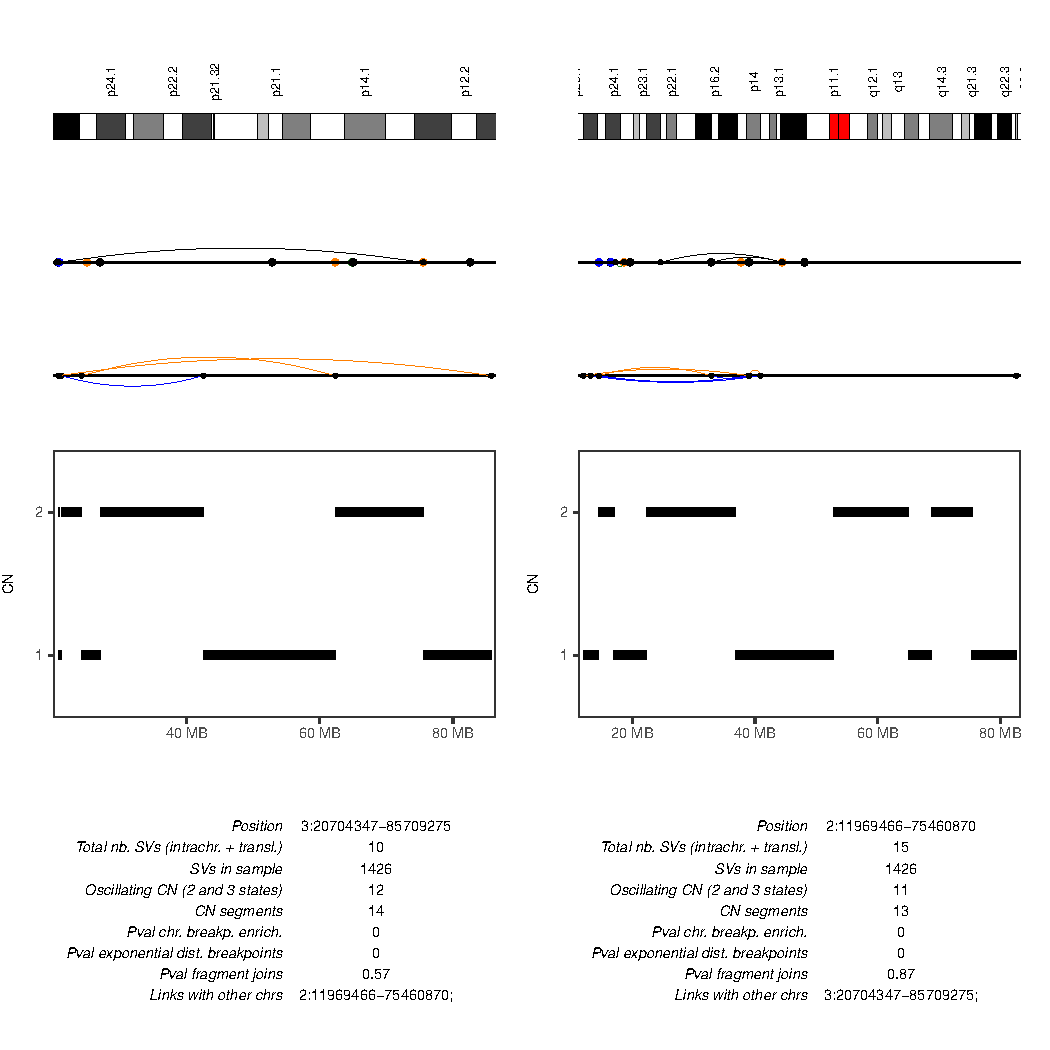
\includegraphics[width=0.85\linewidth,height=0.55\textheight]{figure/unnamed-chunk-10-1} 

}

\caption[Chromothripsis regions detected in patient DO17373 in chromosomes 2 and 3]{Chromothripsis regions detected in patient DO17373 in chromosomes 2 and 3.}\label{fig:unnamed-chunk-10}
\end{figure}


\end{knitrout}

The plots can also be combined into a grid of e.g. four plots and saved to a file:



\section{Bibliography}
\printbibliography
\end{document}


